% This file was created by matlab2tikz.
%
%The latest updates can be retrieved from
%  http://www.mathworks.com/matlabcentral/fileexchange/22022-matlab2tikz-matlab2tikz
%where you can also make suggestions and rate matlab2tikz.
%
\definecolor{mycolor1}{rgb}{0.00000,0.44700,0.74100}%
%
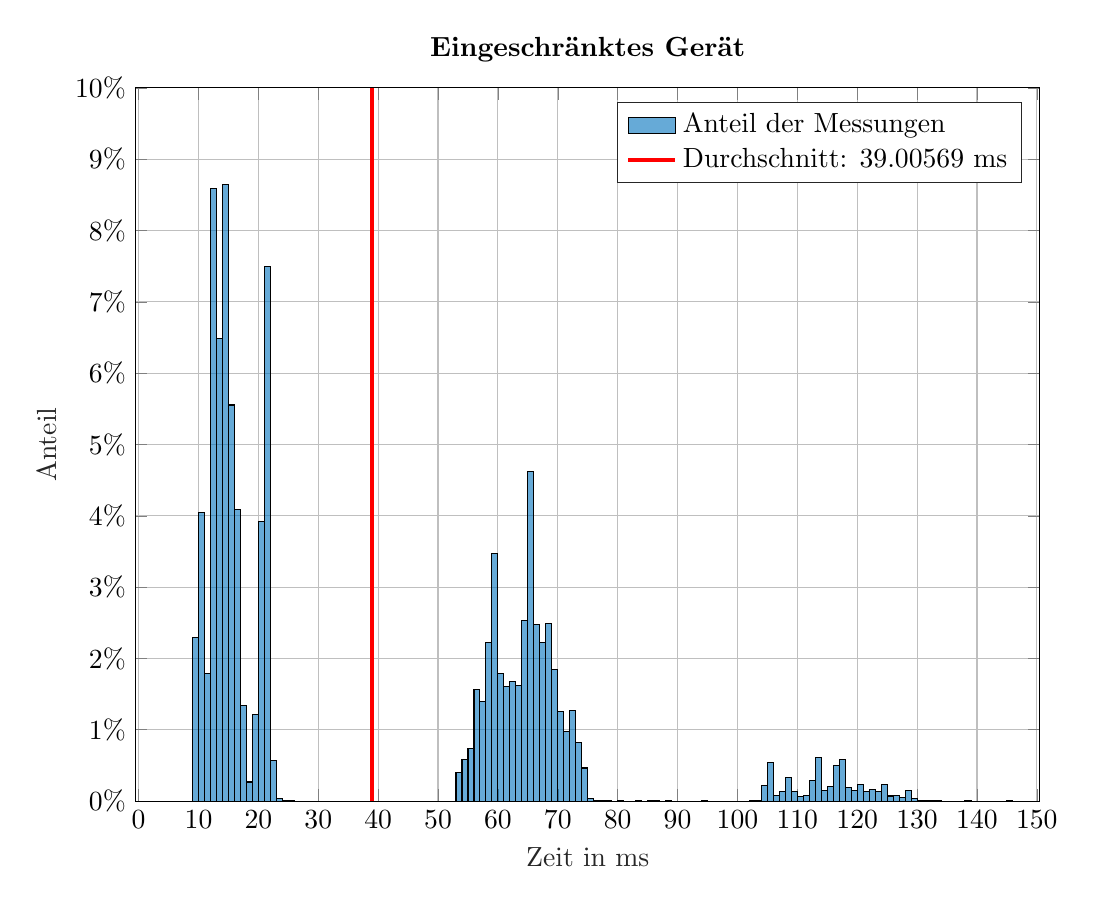
\begin{tikzpicture}

\begin{axis}[%
width=4.521in,
height=3.566in,
at={(0.758in,0.481in)},
scale only axis,
xmin=-0.5,
xmax=150.5,
xtick={  0,  10,  20,  30,  40,  50,  60,  70,  80,  90, 100, 110, 120, 130, 140, 150},
xlabel style={font=\color{white!15!black}},
xlabel={Zeit in ms},
ymin=0,
ymax=0.1,
ytick={0,0.01,0.02,0.03,0.04,0.05,0.06,0.07,0.08,0.09,0.1},
yticklabels={{0\%},{1\%},{2\%},{3\%},{4\%},{5\%},{6\%},{7\%},{8\%},{9\%},{10\%}},
ylabel style={font=\color{white!15!black}},
ylabel={Anteil},
axis background/.style={fill=white},
title style={font=\bfseries},
title={Eingeschr{\"a}nktes Ger{\"a}t},
xmajorgrids,
ymajorgrids,
legend style={legend cell align=left, align=left, draw=white!15!black}
]
\addplot[ybar interval, fill=mycolor1, fill opacity=0.6, draw=black, area legend] table[row sep=crcr] {%
x	y\\
9	0.022931285581888\\
10	0.0404077849860982\\
11	0.0178736925724878\\
12	0.0858466834370449\\
13	0.0649013636965444\\
14	0.0864292334171852\\
15	0.0555276049251953\\
16	0.0409108963325831\\
17	0.0133456904541242\\
18	0.0026744339997352\\
19	0.0121805904938435\\
20	0.0392162054812657\\
21	0.0749900701707931\\
22	0.00574606116774791\\
23	0.000344234079173838\\
24	2.64795445518337e-05\\
25	2.64795445518337e-05\\
26	0\\
27	0\\
28	0\\
29	0\\
30	0\\
31	0\\
32	0\\
33	0\\
34	0\\
35	0\\
36	0\\
37	0\\
38	0\\
39	0\\
40	0\\
41	0\\
42	0\\
43	0\\
44	0\\
45	0\\
46	0\\
47	0\\
48	0\\
49	0\\
50	0\\
51	0\\
52	0\\
53	0.00394545213822322\\
54	0.00577254071229975\\
55	0.0073877929299616\\
56	0.0155964517410301\\
57	0.0139282404342645\\
58	0.0222692969680921\\
59	0.0347411624520058\\
60	0.0178472130279359\\
61	0.0160730835429631\\
62	0.0168145107904144\\
63	0.0162319608102741\\
64	0.0252879650470012\\
65	0.0462597643320535\\
66	0.0247318946114127\\
67	0.0221898583344366\\
68	0.0248907718787237\\
69	0.0185092016417318\\
70	0.0125248245730173\\
71	0.00979743148417847\\
72	0.012736660929432\\
73	0.00815569972196478\\
74	0.0046339202965709\\
75	0.000397193168277506\\
76	7.94386336555011e-05\\
77	2.64795445518337e-05\\
78	2.64795445518337e-05\\
79	0\\
80	5.29590891036674e-05\\
81	0\\
82	0\\
83	2.64795445518337e-05\\
84	0\\
85	2.64795445518337e-05\\
86	2.64795445518337e-05\\
87	0\\
88	2.64795445518337e-05\\
89	0\\
90	0\\
91	0\\
92	0\\
93	0\\
94	2.64795445518337e-05\\
95	0\\
96	0\\
97	0\\
98	0\\
99	0\\
100	0\\
101	0\\
102	5.29590891036674e-05\\
103	7.94386336555011e-05\\
104	0.00222428174235403\\
105	0.00534886799947041\\
106	0.000820865881106845\\
107	0.00132397722759169\\
108	0.00325698397987555\\
109	0.00137693631669535\\
110	0.000582549980140342\\
111	0.000741427247451344\\
112	0.00293922944525354\\
113	0.00609029524692175\\
114	0.00145637495035085\\
115	0.0020389249304912\\
116	0.00500463392029657\\
117	0.00582549980140342\\
118	0.00188004766318019\\
119	0.00142989540579902\\
120	0.0023566794651132\\
121	0.00140341586124719\\
122	0.00164173176221369\\
123	0.00135045677214352\\
124	0.0022772408314577\\
125	0.00071494770289951\\
126	0.000794386336555011\\
127	0.000529590891036674\\
128	0.00142989540579902\\
129	0.000397193168277506\\
130	2.64795445518337e-05\\
131	5.29590891036674e-05\\
132	2.64795445518337e-05\\
133	2.64795445518337e-05\\
134	0\\
135	0\\
136	0\\
137	0\\
138	5.29590891036674e-05\\
139	0\\
140	0\\
141	0\\
142	0\\
143	0\\
144	0\\
145	2.64795445518337e-05\\
146	2.64795445518337e-05\\
};
\addlegendentry{Anteil der Messungen}

\addplot [color=red, line width=1.5pt]
  table[row sep=crcr]{%
39.0056931020786	0\\
39.0056931020786	0.1\\
};
\addlegendentry{Durchschnitt: 39.00569 ms}

\end{axis}
\end{tikzpicture}%